\documentclass[12pt]{beamer}

\usepackage{cmap}
\usepackage[english, russian]{babel}

\usetheme{metropolis}
\usepackage{appendixnumberbeamer}

\usepackage{booktabs}
\usepackage[many]{tcolorbox}

\usepackage{listings}
\lstset{basicstyle=\ttfamily\small,
	showstringspaces=false,
	breaklines=true,
	frame=lrtb,
	% numbers=left,
	extendedchars=\true,
	language=bash
}

\usepackage{xspace}
\newcommand{\themename}{\textbf{\textsc{metropolis}}\xspace}
% \setsansfont{Fira Sans Bold}

\title{Автоматизация миграции программного кода на новый набор библиотек}
% \subtitle{A modern beamer theme}
\date{\today}
\author{Артем Алексюк}
\institute{Санкт-Петербургский политехнический университет Петра Великого}
% \titlegraphic{\hfill
\includegraphics[height=1.5cm]{logo.pdf}}

\newtcolorbox{mybox}[1][]{
    width=\textwidth,
    arc=3mm,
%    auto outer arc,
    boxsep=0cm,
    toprule=1pt,
    leftrule=1pt,
    bottomrule=1pt,
    rightrule=1pt,
    colframe=white,
    boxrule=0pt,frame hidden,
    breakable,
    nobeforeafter,
    enhanced jigsaw,
    opacityframe=0.7,
    fontupper=\bfseries,
    opacityback=0.7
}

% \setbeamertemplate{blocks}[rounded][shadow=false]
% \addtobeamertemplate{block begin}{\pgfsetfillopacity{0.5}}{\pgfsetfillopacity{1}}

\begin{document}

\maketitle

%\begin{frame}{Table of contents}
%  \setbeamertemplate{section in toc}[sections numbered]
%  \tableofcontents[hideallsubsections]
%\end{frame}

% \section{Introduction}


{
\usebackgroundtemplate{%
\tikz\node[opacity=0.4]{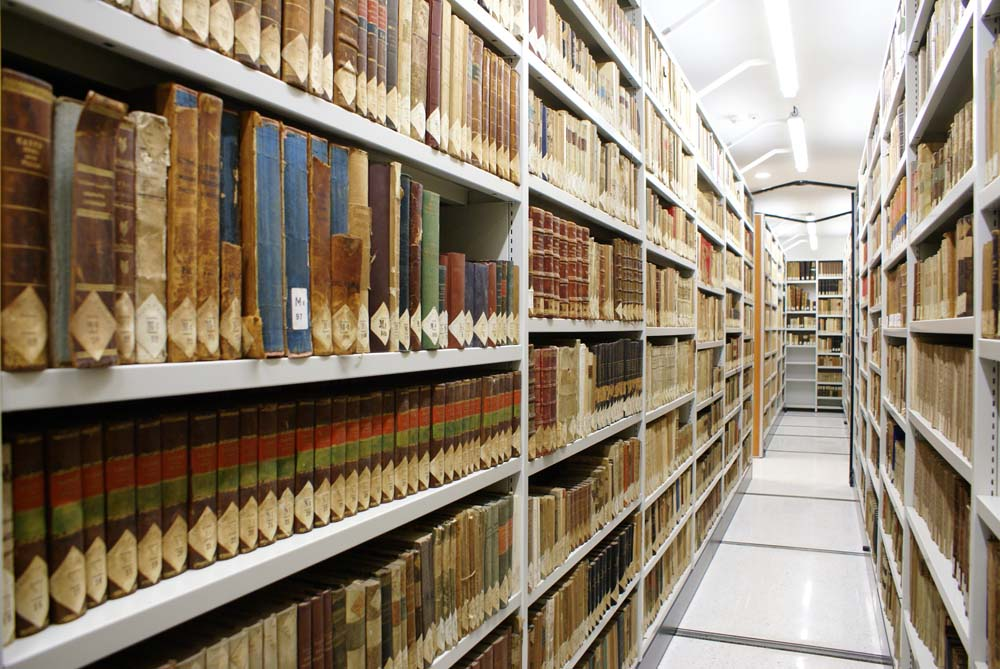
\includegraphics[height=\paperheight,width=\paperwidth]{historical-archive.jpg}};}
\begin{frame}{Актуальность}
\begin{mybox}[]
Миграция в новое библиотечное окружение?
\begin{itemize}
	\item Новая программная платформа
	\item Новая аппаратная платформа
	\item Унаследованный код, несовместимый с современными системами, средствами разработки, библиотеками
\end{itemize}
\end{mybox}
\end{frame}
}

{
\usebackgroundtemplate{%
\tikz\node[opacity=0.4]{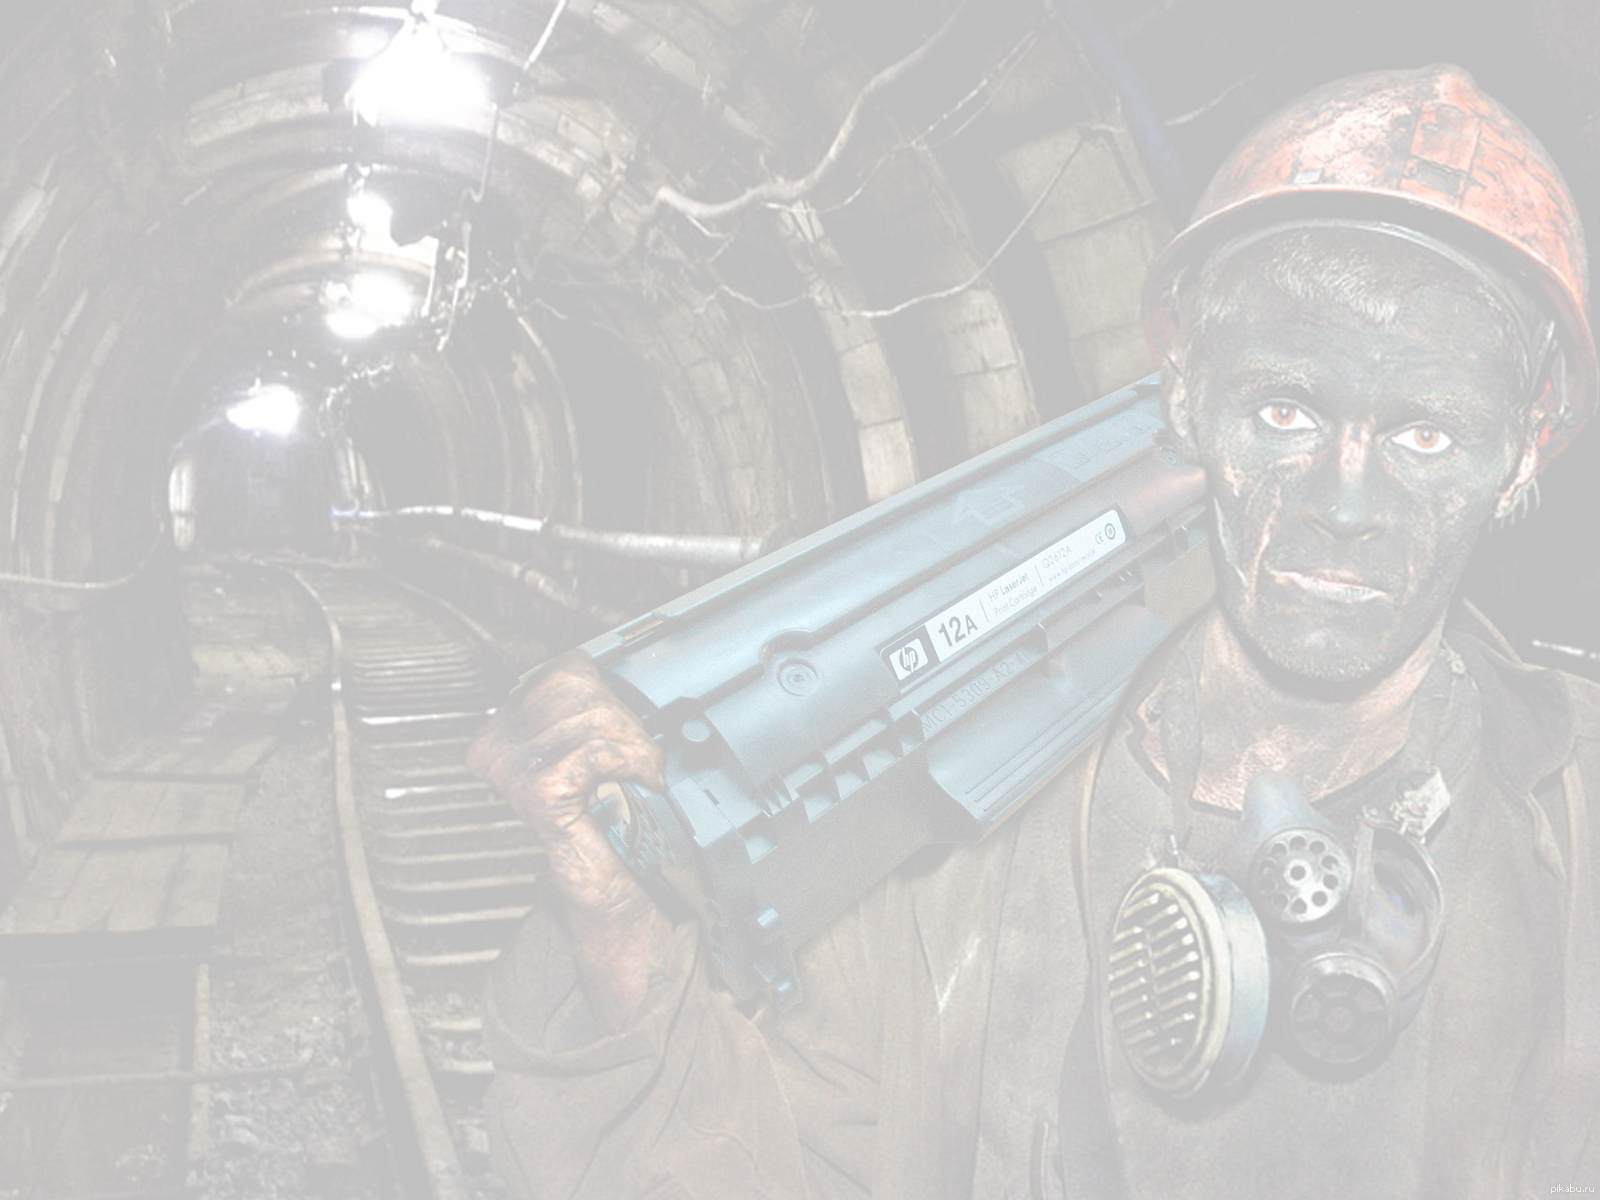
\includegraphics[height=\paperheight,width=\paperwidth]{miner2.jpg}};}
\begin{frame}{Сложности}
\begin{mybox}[]
\begin{itemize}
	\item Практически всегда миграция идет вручную
	\item Много рутинной работы $\Longrightarrow$ высокая вероятность допустить ошибку
	\item Попробовать автоматизировать?
\end{itemize}
\end{mybox}
\end{frame}
}

{
\usebackgroundtemplate{%
\tikz\node[opacity=0.4]{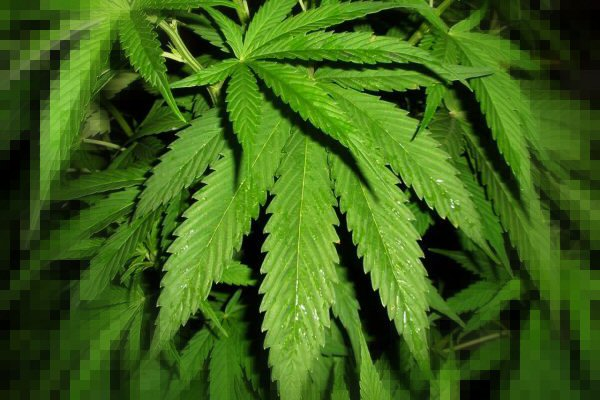
\includegraphics[height=\paperheight,width=\paperwidth]{plan.jpg}};}
\begin{frame}{Общий подход к решению задачи}
\begin{mybox}[]
\begin{itemize}
	\item Создать модели используемых библиотек
	\item Модель - частная спецификация, описывающая внешнее поведение библиотеки
	\item Проанализировать модели, найти 
	\item Преобразовать изменения обратно в код
\end{itemize}
\end{mybox}

\metroset{block=fill}
\begin{alertblock}{Почему модели, а не сам код?}
Удобнее анализировать декларативные модели, чем императивный код
\end{alertblock}
\end{frame}
}

{
\usebackgroundtemplate{%
\tikz\node[opacity=0.4]{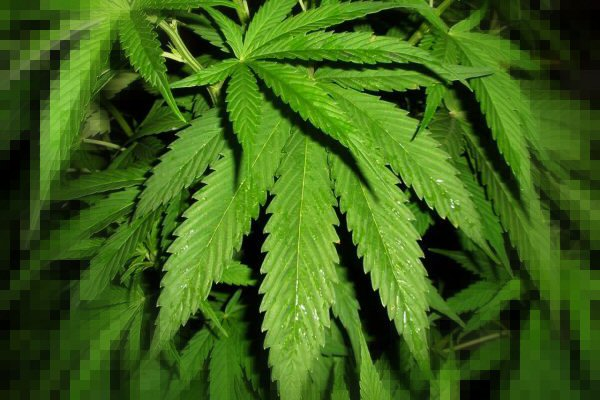
\includegraphics[height=\paperheight,width=\paperwidth]{plan.jpg}};}
\begin{frame}{Спецификация библиотек}
\begin{mybox}[]
	Уже есть языки для описания библиотек (например, IDL для RPC), но они не содержат семантическую информацию.
	Разрабатываемая модель библиотеки должна:
\begin{itemize}
	\item Детально описывать внешний интерфейс библиотеки;
	\item Задавать возможные протоколы использования библиотеки;
	\item Специфицировать побочные действия библиотеки – влияние ее на окружение;
	\item Явно вводить семантические описания поведения библиотек.
\end{itemize}
\end{mybox}
\end{frame}
}

\begin{frame}[fragile]{Формализм}
  \begin{mybox}[]
  \begin{itemize}
  	\item Для описания моделей используются расширенные конечные автоматы:
  	$A = <Q, Q_0, X, V, C, T>$
  	
  	C - множество стимулов (например, вызовов функций), $С_i$ – появление i-ой стимула
  	
  	$C_i^A$ - множество семантических действий, инициируемых запуском функции при условии истинности $C_i^{CondA}$
  	
  	$C_i^D$ - множество дочерних автоматов, запускаемых функцией при условии $C_i^{CondD}$;
  \end{itemize}
  \end{mybox}
\end{frame}

% \section{Titleformats}

\begin{frame}{Пример автомата}
	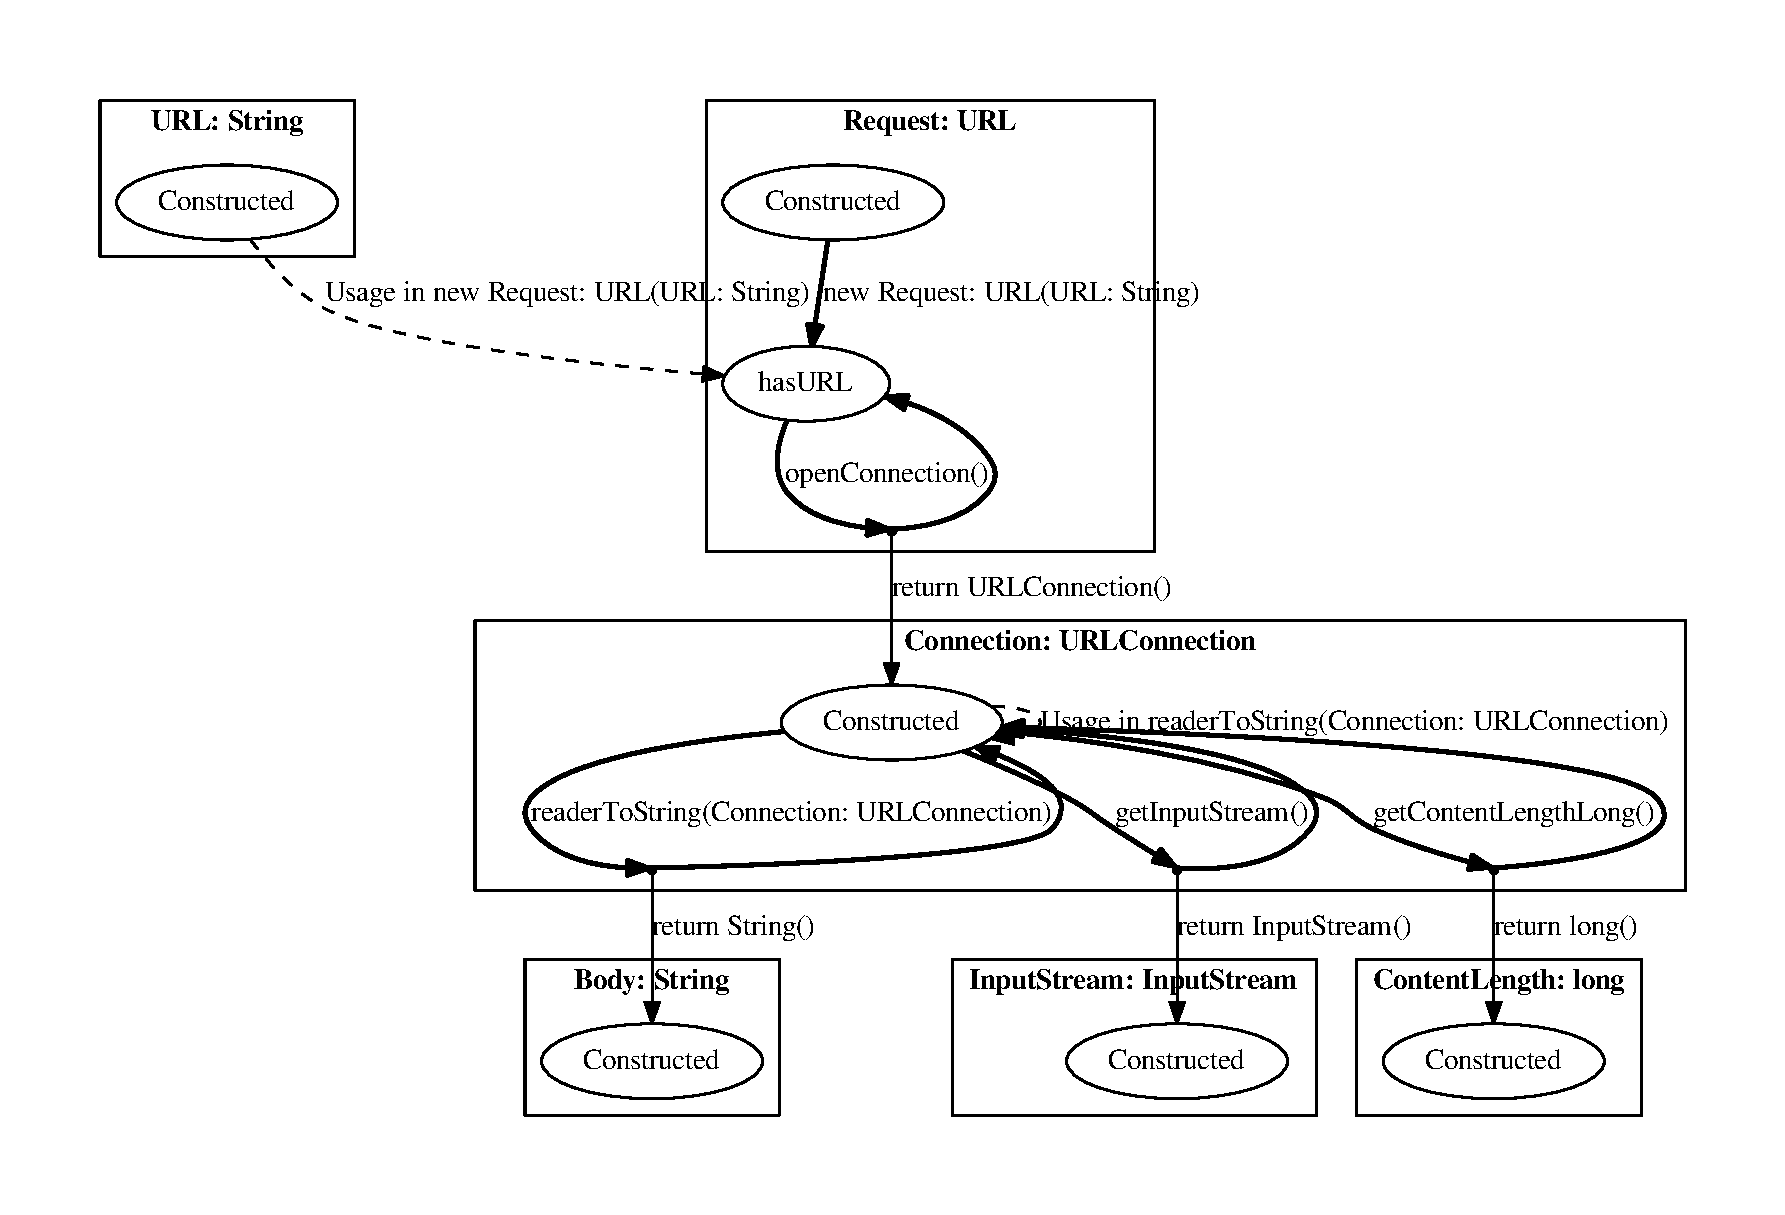
\includegraphics[width=\textwidth]{java.pdf}
\end{frame}

\begin{frame}{Пример автомата}
	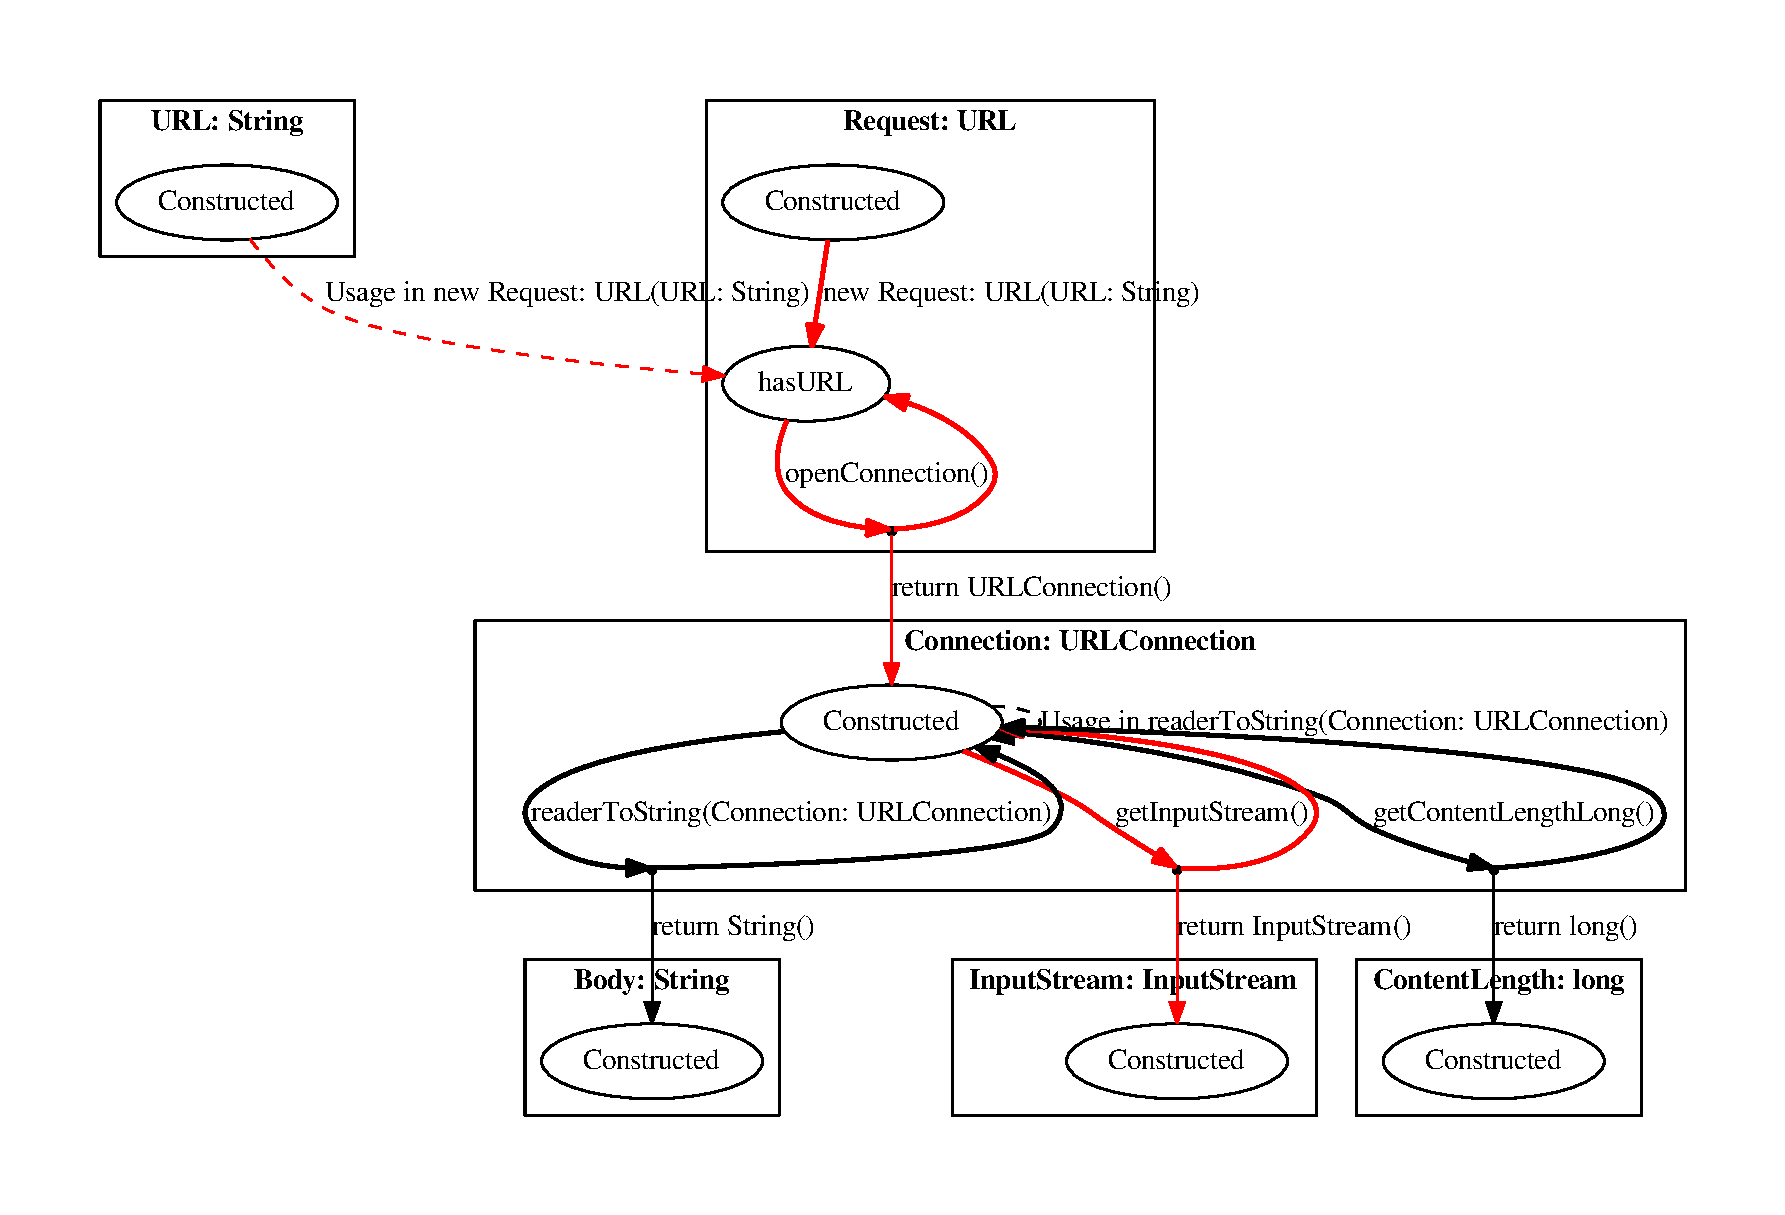
\includegraphics[width=\textwidth]{extracted_java.pdf}
\end{frame}

\begin{frame}[fragile]{Извлечение информации из кода}
  \begin{mybox}[]
  \begin{itemize}
  	\item Статический анализ: используя одно из подходящий представлений программы (CFG, SSA, Def-Use chains), попытаться отобразить порядок действий на модель
  	\item Проблема - иногда нужно знать, какое значение хранится в переменной. Статический анализ не всегда может дать ответ.
  \end{itemize}
  \end{mybox}
\end{frame}


\begin{frame}[fragile]{Извлечение информации из кода}
	\begin{mybox}[]
		\begin{itemize}
			\item Динамический анализ: программа инструментируется, на основе трассы выполнения составляется путь в модели
			\item Для инструментирования используется AOP (аспекты) в реализации AspectJ
			\item Преимущества: проще в реализации, выше точность
			\item Бонус: проверка корректности использования исходной библиотеки
		\end{itemize}
	\end{mybox}
\end{frame}


\begin{frame}[fragile]{Поиск соответствия между моделями}
  \begin{mybox}[]
  \begin{itemize}
  	\item При переносе необходимо сохранить:
  	  \begin{itemize}
  	  	\item Набор действий, совершенных над библиотекой
  	  	\item Зависимости по данным
  	  \end{itemize}
  	\item Первые версии инструмента: модель преобразуется в граф, с помощью алгоритма Дейкстры ищем кратчайший путь между вершинами
  	\item Сейчас: используется волновой алгоритм, в поисках более эффективных алгоритмов
  \end{itemize}
  \end{mybox}
\end{frame}

\begin{frame}[fragile]{Текущее состояние}
  \begin{mybox}[]
  \begin{itemize}
  	\item Модель библиотеки, где можно описать состояния, связи и прототипы функций.
  	\item Описание моделей с помощью DSL на Kotlin
  	\item Инструмент для миграции программ на языке Java
  	\item Система проверки корректности преобразования
  \end{itemize}
  \end{mybox}
\end{frame}

\begin{frame}[fragile]{Пример миграции}
До:
\begin{lstlisting}
URL url = new URL("http://api.ipify.org/");
URLConnection conn = url.openConnection();
if (conn.getContentLengthLong() > 0) {
    String response = new BufferedReader(new InputStreamReader(conn.getInputStream())).lines().collect(Collectors.joining("\n"));
    System.out.println(response);
} else {
    System.out.println("Error!");
}
\end{lstlisting}
\end{frame}

\begin{frame}[fragile]{Пример миграции}
После:
\begin{lstlisting}[basicstyle=\ttfamily\scriptsize]
HttpGet url = new HttpGet("http://api.ipify.org/");
CloseableHttpClient newMachine_Client_0 = HttpClients.createDefault();
CloseableHttpResponse conn = newMachine_Client_0.execute(url);
long linkedEdge_ContentLength_1 = conn.getEntity().getContentLength();
if (linkedEdge_ContentLength_1 > 0) {
    InputStream linkedEdge_InputStream_2 = conn.getEntity().getContent();
    String response = new BufferedReader(new InputStreamReader(linkedEdge_InputStream_2)).lines().collect(Collectors.joining("\n"));
    System.out.println(response);
} else {
    System.out.println("Error!");
}
\end{lstlisting}
\end{frame}

\begin{frame}[fragile]{Дальнейшее развитие}
	\begin{mybox}[]
		\begin{itemize}
			\item Улучшение алгоритма поиска соответствия, повышение производительности + увеличение возможностей
			\item Проектирование языка для описания моделей (сейчас это ad-hoc решение)
			\item Поиск способа задания соответствия между семантическими доменами
			\item Увеличение количества информации, содержащейся в моделях
		\end{itemize}
	\end{mybox}
\end{frame}

\end{document}
